\chapter{Text as Data}
\label{chap:dtm}

\begin{abstract}{Abstract}
  This chapter shows how you can analyze texts that are stored as a data frame column or variable using functions from the package \pkg{quanteda} in R and the package \pkg{sklearn} in Python in Python and R.
  Please see \refchap{protext} for more information on reading and cleaning text.
  
\end{abstract}

\keywords{Text as Data, Document-Term Matrix}

\begin{objectives}
\item Create a document-term matrix from text
\item Perform feature and document selection and weighting
\item Understand and use more advanced representations such as n-grams and embeddings
\end{objectives}

\section{The bag of words and term-document matrix}
\label{sec:dtm}

Before you can analyse text using the computer, the text must be represented in a way that is understandable for the computer.

The Document-term matrix (DTM, also called the term-document matrix or TDM) is a common numerical representation of text.
This represents a \concept{corpus} (or set of documents) as a matrix or table, where each row represents a document, each column represents a term (word),
and the numbers in each cell show how often that word occurs in that document.

\pyrex[caption=Example document-term matrix,output=r,format=table]{ch_dtm/dtm}

As an example, \refex{dtm} shows a DTM made from two lines from the famous poem by Mary Angelou.
The resulting matrix has two rows, one for each line; and 11 columns, one for each unique term (word).
In the columns you see the document frequencies of each term: the word ``bird'' occurs once in each line,
but the word ``with'' occurs only in the first line (text1) and not in the second (text2).

In R, you can use the \fn{dfm} function from the \pkg{quanteda} package.
This function can take a vector or column of texts and transforms it directly into a DTM.
In Python, you achieve the same by creating an object of the \cls{CountVectorizer} class, which has a \fn{fit\_transform} function.


\subsection{Tokenization}

In order to turn a corpus into a matrix, each text needs to be \concept{tokenized},
meaning that it must be split into a list (vector) of words.
This seems trivial, as English (and most western) text generally uses spaces to demarcate words.
However, even for English there are a number of edge cases. 
For example, should `haven't' be seen as a single word, or two?

\pyrex[caption=Differences between tokenizers]{ch_dtm/tokenize}

\refex{tokenize} shows how Python and R deal with the sentence ``I haven't seen John's derring-do''.
For Python, we first use |CountVectorizer.build_tokenizer| to access the built-in tokenizer.
As you can see in the first line of input, this tokenizes ``haven't'' to |haven|,
which of course has a radically differeny meaning. Moreover, it silently drops all single-letter words,
including the |'t|, |'s|, and |I|.
A more reasonable tokenizer is the \cls{TreebankWordTokenizer} included in the \pkg{nltk} package, which contains a number of functions for doing natural language processing in python.
This tokenizer splits ``haven't'' into |have| and |n't|, which is a reasonable outcome.
Unfortunately, this tokenizer assumes that text has already been split into sentence,
and it also includes punctuation as tokens by default.
For this reason, we introduce a custom tokenizer based on the Treebank tokenizer,
which splits text into sentences (using \fn{nltk.sent\_tokenize}) and allows for a custom criterion for keeping tokens,
in this case that the token must contain at least one letter. 

For R, we simply call the \fn{tokens} function from the \quanteda\ package.
This keeps |haven't| and |John's| as a single word, which is probably less desirable than splitting the words
but at least better than outputting the word |haven|.

As this simple example shows, even a relatively simple sentence is tokenized differently by the three tokenizers considered here.
Depending on the research question, these differences might or might not be important.
However, it is always a good idea to check the output of this (and other) preprocessing steps so you understand
what information is kept or discarded.

% Listings won't work with the japanese output, so I manually created png. Sorry!
\begin{ccsexample}
  \doublecodex{ch_dtm/haiku}
  \begin{tcbraster}[raster columns=2,raster equal height=rows,raster valign=top]
  \begin{tcolorbox}[title=Python Output]
      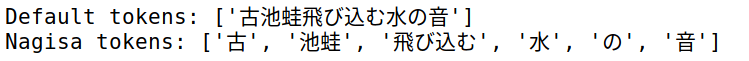
\includegraphics[width=\linewidth]{{ch_dtm/haiku.py}.png}
  \end{tcolorbox}%
  \begin{tcolorbox}[title=R Output]
      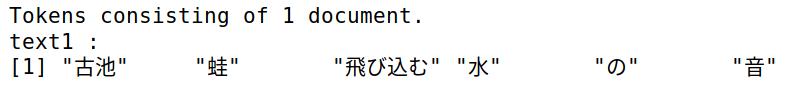
\includegraphics[width=\linewidth]{{ch_dtm/haiku.r}.png}
  \end{tcolorbox}%
\end{tcbraster}
  \caption{Tokenization of Japanese verse}\label{ex:haiku}
\end{ccsexample}



Note that for languages such as Chinese, Japanese, and Korean, which do not use spaces to delimit words, the story is more difficult.
Although a full treatment is beyond the scope of this book, \refex{haiku} shows a small example of tokenizing Japanese text,
in this case the famous haiku ``the sound of water'' by Bash\={o}.
The default tokenizer in quanteda actually does a good job, in contrast to the default python tokenizer
that simply keeps the whole string as one word
(which makes sense since this tokenizer only looks for whitespace or punctuation).
For python the best bet is to use a custom package for tokenizing Japanese, such as the \pkg{nagisa} package.
This package contains a tokenizer which is able to tokenize the Japanese text, and we could use this in the \cls{CountVectorizer}
much like we used the \cls{TreebankWordTokenizer} for English earlier.
Similarly, with heavily inflected languages such as Hungarian or Arabic,
it might be better to use preprocessing tools developed specifically for these languages, but treating those is unfortunately
beyond the scope of this book. 


\subsection{The DTM as a Sparse Matrix}

\pyrex[caption=Example document-term matrix]{ch_dtm/sotu}

\refex{sotu} shows a more realistic example.
It downloads all US 'State of the Union' speeches and creates a document-term matrix from them.
Since the matrix is now easily too large to print, both python and R simply list the size of the matrix.
R lists $85$ documents (rows) and $17,999$ features (columns), and Python reports that it's size is $85\times22219$.
Note the difference in the amount of columns (unique terms) due to the differences in tokenization as discussed above. 

\pyrex[caption=A look inside the DTM]{ch_dtm/freq}
\pyrex[caption=A look inside the DTM]{ch_dtm/freq2}

In \refex{freq} we show how you can look at the contents of the DTM. First, we show the overall term and document frequencies of each word, where we showcase words at different frequencies. Unsurprisingly, the word \emph{the} tops both charts, but further down there are minor differences.
In all cases, the highly frequent words are mostly functional words like \emph{them} or \emph{first}. More informative words such as \emph{investments} are by their nature used much less often.
Such term statistics are very useful to check for noise in the data and get a feeling of the kind of language that is used. 
Second, we take a look at the frequency of these same words in four speeches from Truman to Obama. All use words like \emph{the} and \emph{first}, but none of them talk about \emph{defrauded} -- which is not surprising, since it was only used once in all the speeches in the corpus.

However, the words that ranked around 1,000 in the top frequency are still used in less than half of the documents.
Since there are about 17,000 even less frequent words in the corpus, you can imagine that most of the document-term matrix consists of zeroes. 
The output also noted this \concept{sparsity} in the first output above.
In fact, R reports that the dtm is $91\%$ sparse, meaning that percentage of all entries is zero.
Python reports a similar figure, namely that there are only just under 150 thousand non-zero entries
out of a possible $8\times22219$, which boils down to a 92\% sparse matrix.

Note that to display the matrix we turned it from a \concept{sparse matrix} representation into a \concept{dense matrix}.
Briefly put, in a dense matrix, all entries are stored as a long list of numbers, including all the zeroes.
In a sparse matrix,  only the non-zero entries and their location are stored. 
This conversion (using the function \verb|as.matrix| and \verb|todense| respectively), however, was only performed after selecting a small subset of the data.
In general,  it is very inefficient to store and work with the matrix in a \concept[dense matrix]{dense} format.
For a reasonably large corpus with tens of thousands of documents and different words, this can quickly run billions of numbers,
which can cause problems even on modern computers and is moreover very inefficient.
With sparsities of often above 99\%, using a sparse matrix representation can easily reduce storage requirements by a hundred times and in the process speed up calculations by reducing the number of entries that need to be inspected.
Both \quanteda\ and \sklearn\ store DTMs as sparse matrices by default,
and most analysis tools are able to deal with sparse matrices very efficiently.
(but see \refsec{workflow} for problems with machine learning on sparse matrices in R). 

A final note on the difference between python and R in this example.
The code in R is much simpler and produces nicer results since it also shows the words and the speech names.
In python, we wrote our own helper function to create the frequency statistics which is built into the R \quanteda\ package.
These differences between Python and R reflect a pattern that is true in many (but not all) cases:
In python libraries such as \numpy\ and \sklearn\ are setup to maximize performance,
while in R a library such as \quanteda\ or \tidyverse\ is more geared towards ease of use.
For that reason, the DTM in python does not `remember' the actual words, it uses the index of each word,
so it consumes less memory if you don't need to use the actual words in e.g. a machine learning setup.
R, on the other hand, stores the words and also the document IDs and metadata in the DFM object.
This is easier to use if you need to look up a word or document, but it consumes (slightly) more memory. 


\begin{feature}
  \textbf{R: Why is it a document-feature matrix?}
The package \pkg{quanteda} uses the term document-feature matrix because the columns can also contain
other information instead of terms, such as word pairs, and these are collectively called \emph{features} of the text.
\end{feature}

\begin{feature}
\noindent\textbf{Python: Why fit\_transform?}
In Python, you don't have a function that directly transforms text into a DTM.
Instead, you create an \emph{transformer} called a CountVectorizer,
which can then be used to 'vectorize' texts (turn it into a row of numbers)
by counting how often each word occurs.
This uses the \fn{fit\_transform} function which is offered by all \sklearn\ transformers.
It `fits' the model on the training data, which in this case means learning the vocabulary.
It can then be used to transform other data into a DTM with the exact same columns,
which is often required for algorithms.
Because the feature names (the words themselves) are stored in the CountVectorizer
rather than the document-term matrix, you generally need to keep both objects.
\end{feature}

\subsection{The DTM as a `bag of words'}


As you can see already in these simple examples, the document-term matrix discards quite a lot of information from text.
Specifically, it disregards the order or words in a text: `John fired Mary' and `Mary fired John' both result in the same DTM,
even though the meaning of the sentences is quite different.
For this reason, a DTM is often called a \concept{bag of words}, in the sense that all words in the document are simply put in a big bag
without looking at the sentences or context of these words. 

Thus, the DTM can be said to be a specific and `lossy' representation of the text, that turns out to be quite useful for certain tasks:
The frequent occurrence of words like ``employment'', ``great'', or ``I'' might well be good indicators that a text is about the economy,
is positive, or contains personal expressions respectively.
As we will see in the next chapter, the DTM representation can be used for many different text analyses, from dictionaries to supervised and unsupervised machine learning.

Sometimes, however, you need information that is encoded in the order of words.
For example, in analysing conflict coverage it might be quite important to know who attacks whom, not just that attacking took place.
In the last section of this chapter we will look at some ways to create a richer matrix-representation by using word pairs.
Although it is beyond the scope of this book,
you can also use automatic syntactic analysis to take grammatical relations into account as well.
As is always the case with automatic analyses, it is important to understand what information the computer is looking at,
as the computer cannot find patterns in information that it doesn't have.

\subsection{The (unavoidable) Word Cloud}

One of the most famous text visualizations is without doubt the word cloud.
Essentially, a word cloud is an image where each word is displayed in a size that is representative of its frequency.
Depending on preference, word position and colour can be random, depending on word frequency, or in a decorative shape.

Word Clouds are often criticised since they are (sometimes) pretty but mostly not very informational.
The core reason for that is that only a single aspect of the words is visualized (frequency),
and simple word frequency is often not that informative: the most frequent words are generally uninformative `stop words' like ``the'' and ``I''.

For example, \refex{wordcloud} shows the word cloud for the state of the union speeches downloaded above.
In R, this is done using the \quanteda\ function \fn{textplot\_wordcloud}.
In Python we need to work a little harder, since it only has the counts, not the actual words.
So, we sum the DTM columns to get the frequency of each word, and combine that with the feature names (words)
from the |CountVectorized| object |cv|. Then we can create the WordCloud and give it the frequencies to use.
Finally, we plot the cloud and remove the axes.

\pyrex[caption=Word Cloud of the US State of the Union corpus,format=png]{ch_dtm/wordcloud}

The results from Python and R look different at first -- for one thing, R is nice and round but Python has more colors!
However, if you look at the cloud you can see both are not very meaningful: the largest words are all punctuation or words like
`a', `and', or `the'.
You have to look closely to find words like `federal' or `security' that give a hint on what the texts were actually about.



\section{Weighting and selecting documents and terms}
\label{sec:dtmselect}

\subsection{Stopword removal}

\subsection{Trimming a DTM}


\subsection{Weighting a DTM}


\section{Advanced representation of text}
\label{ngram}

The examples above all created document-term matrices where each column actually represents a word.
There is more information in a text, however, than pure word counts.
The phrases: \emph{the movie was not good, it was in fact quite bad} and \emph{the movie was not bad, in fact it was quite good}
have exactly the same word frequencies, but are quite different in meaning.
Similarly, \emph{the new residents of York} and \emph{the residents of New York} are talking about quite different people. 

Of course, in the end which aspect of the meaning of a text is important depends on your research question:
if you want to know the sentiment about the movie, it is important to take a word like `not' into account;
but if you are interested in the topic or genre of the review, or the extremity of the language used, this might not be relevant.

The core idea of this section is that in many cases this information can be captured in a DTM by having the columns represent different information than just words, for example word combinations or groups of related words.
This is often called \concept{feature engineering}, as we are using our domain expertise to find the right features (columns, independent variables) to capture the relevant meaning for our research question.
If we are using other columns than words it is also technically more correct to use the name \concept{Document-feature matrix}, as \quanteda\ does, but we will stick to the most common name here and simply continue using the name DTM.

\subsection{N-grams}

The first feature we will discuss are n-grams.
The simplest case is a bigram (or 2-gram), where each feature is a pair of adjacent words.
The example used above, \emph{the movie was not bad}, will yield the following bigrams: \emph{the-movie}, \emph{movie-was}, \emph{was-not}, and \emph{not-bad}.
Each of those bigrams is then treated as a feature, that is, a DTM would contain one column for each word pair.

As you can see in this example, we can now see the difference between \emph{not-bad} and \emph{not-good}.
The downside of using n-grams is that there are many more unique word pairs than unique words,
so the resulting DTM will have many more columns.
Moreover, there is a bigger \concept{data scarcity problem}, as each of those pairs will be less frequent,
making it more difficult to find sufficient examples of each to generalize over.

Although bigrams are the most frequent use case, trigrams (3-grams) and (rarely) higher-order n-grams can also be used.
As you can imagine, this will create even bigger DTMs and worse data scarcity problems,
so require even more attention paid to feature selection and/or trimming.


\pyrex[caption=Generating n-grams]{ch_dtm/ngram}

\refex{ngram} shows how n-grams can be created and used in Python and R.
In Python, you can pass the \verb|ngram=(n, m)| option to the vectorizer,
while R has a \verb|tokens_ngrams(n:m)| function.
Both will post-process the tokens to create all n-grams in the range of n to m.
In this example, we are asking for unigrams (i.e., the words themselves), bigrams and trigrams of a simple example sentence.
Both languages produce the same output, with R separating the words with an underscore while python uses a simple space.

\pyrex[caption=Words and bigrams containing 'government',output=r,format=table]{ch_dtm/ngram2}

\refex{ngram2} shows how you can generate n-grams for a whole corpus.
In this case, we create a DTM of the state of the union matrix with all bigrams included.
A glance at the frequency table for all words containing \emph{government} shows that,
besides the word itself and it's plural and possessive forms, the bigrams include compound words (federal and local government),
phrases with  the government as subject (the government can and must), and nouns for which the government is an adjective
(government spending and government programs).

You can imagine that including all these words as features will add many possibilities for analysis of the DTM
which would not be possible in a normal bag-of-words approach.
The terms local and federal government can be quite important to understand policy positions,
but for e.g. sentiment analysis a bigram like \emph{not good} would also be insightful
(but make sure 'not' is not on your stop word list!).   

\subsection{Collocations}

A special case of n-grams are collocations.
In the strict corpus linguistic sense of the word, collocations are pairs of words that occur more frequently than expected
based on their underlying occurence.
For example, the phrase \emph{crystal clear} presumably occurs much more often than would be expected by chance given
how often \emph{crystal} and \emph{clear} occur separately.
Collocations are important for text analysis since they often have a specific meaning,
for example because they refer to names such as \emph{New York} or disambiguate a term like \emph{sound} in \emph{sound asleep},
a \emph{sound proposal}, or \emph{loud sound}.

\refex{colloc} shows how to identify the most `surprising' collocations using R and Python.
For Python, we use the \pkg{gensim} package which we will also use for topic modeling in \refsec{unsupervised}.
This package has a \cls{Phrases} class which can identify the bigrams in a list of tokens.
In R, we use the \fn{textstat\_collocations} function from \quanteda.
These packages each use a different implementation: \pkg{gensim} uses pointwise mutual information, i.e.
how much information about finding the second word does seeing the first word give you?
Quanteda estimates an interaction parameter in a loglinear model.
Nonetheless, both methods give very similar results, with Saddam Hussein, the Iron Curtain, Al Qaida, and red tape topping the list for each.


\begin{ccsexample}
\doublecodex{ch_dtm/colloc}
\codexoutputtable{ch_dtm/colloc.r}
\doublecodex{ch_dtm/colloc2}
\codexoutputtable{ch_dtm/colloc2.r}
\caption{Identifying and applying collocations in the US State of the Union}\label{ex:colloc}
\end{ccsexample}


The next block demonstrates how to use these collocations in further processing.
In R, we filter the collocations list on $lambda>8$ and use the \fn{tokens\_compound} function to compound bigrams from that list.
As you can see in the term frequencies filtered on `hussein', the regular terms (apart from the posessive) are removed and the compounded term now has 26 occurrences.
For Python, we use the \cls{PhraseTransformer} class, which is an adaptation of the \cls{Phrases} class to the \sklearn\ methodology.
After setting a standard threshold of 0.7, we can use \fn{fit\_transform} to change the tokens.
The term statistics again show how the individual terms are now replaced by their compound. 


\subsection{Word Embeddings}

A recent addition to the text analysis toolbox are \concept{word embeddings}.
Although it is beyond the scope of this book to give a full explanation of the algorithms behind word embeddings,
they are relatively easy to understand and use at an intuitive level.

The first core idea behind word embeddings is that the meaning of a word can be expressed using a relatively small \concept{embedding vector}, generally consisting of around 300 numbers which can be interpreted as dimensions of meaning.
The second core idea is that these embedding vectors can be derived by scanning the context of each word in millions and millions of documents.


These embedding vectors can then be used as features or DTM columns for further analysis.
Using embedding vectors instead of word frequencies has the advantages of strongly reducing the dimensionality of the DTM:
instead of (tens of) thousands of columns for each unique word we only need hundreds of columns for the embedding vectors.
This means that further processing can be more efficient as fewer parameters need to be fit,
or conversely that more complicated models can be used without blowing up the parameter space.
Another advantage is that a model can also give a result for words it never saw before, as these words most likely will have an embedding vector and so can be fed into the model.
Finally, since words with similar meanings should have similar vectors,
a model fit on embedding vectors gets a `head start' since the vectors for words like `great' and `fantastic' will already be relatively close to each other, while all columns in a normal DTM are treated independently.

\newcommand{\fnglove}{\footnote{The full embedding models can be downloaded from https://nlp.stanford.edu/projects/glove/. To make the file easier to download, we took only the 10,000 most frequent words of the smallest embeddings file (the 50 dimension version of the 6B tokens model). For serious applications you probably want to download the larger files, in our experience the 300 dimension version usually gives good results. Note that the files on that site are in a slightly different format which lacks the initial header line, so if you want to use other vectors for the examples here you can convert them with the \fn{glove2word2vec} function in the \pkg{gensim} package. For R, you can also simply omit the \verb|skip=1| argument as apart from the header line the formats are identical}}

The assumption that words with similar meanings have similar vectors can also be used directly to extract synonyms.
This can be very useful, for example for (semi-)automatically expanding a dictionary for a concept.
\refex{embedding} shows how to download and use pre-trained embedding vectors to extract synonyms.
First, we download a very small subset of the pre-trained Glove embedding vectors\fnglove,
wrapping the download call in a condition to only download it when needed.

Then, for Python, we use the excellent support from the \pkg{gensim} package to load the embeddings into a \cls{KeyedVectors} object.
Although not needed for the rest of the example, we create a pandas DataFrame from the internal embedding values so the internal structure becomes clear: each row is a word, and the columns (in this case 50) are the different (semantic) dimensions that characterize that word according to the embeddings model.
This data frame is sorted on the first dimension, which shows that negative values on that dimension are related to various sports.
Next, we switch back to the \cls{KeyedVectors} object to get the most similar words to the word \emph{fraud}, which is apparently related to similar words like \emph{bribery} and \emph{corruption} but also to words like \emph{charges} and \emph{alleged}.
These similarities are a good way to (semi-)automatically expand a dictionary: start from a small list of words,
find all words that are similar to those words, and if needed manually curate that list.
Finally, we use the embeddings to solve the `analogies' that famously showcase the geometric nature of these vectors:
if you take the vector for \emph{king}, subtract the vector for \emph{man} and add that for \emph{woman},
the closest word to the resulting vector is \emph{queen}.
Amusingly, it turns out that soccer is a female form of football, probably showing the American cultural origin of the source material.

For R, there was less support from existing packages so we decided to use the opportunity to show both the conceptual simplicity of embeddings vectors and the power of matrix manipulation in R.
Thus, we directly read in the word vector file which has a head line and then on each line a word followed by its 50 values.
This is converted to a matrix with the rownames showing the word,
which we normalize to (Euclidean) length of one for each vector for easier processing. 
To determine similarity, we take the cosine distance between the vector representing a word with all other words in the matrix.
As you might remember from algebra, the cosine distance is the dot product between the vectors normalized to have length one
(just like Pearson's product-moment correlation is the dot product between the vectors normalized to z-scores per dimension).
Thus, we can simply multiply the normalized target vector with the normalized matrix to get the similarity scores.
These are then sorted, renamed, and the top values are taken using the basic functions from \refchap{datawrangling}.
Finally, analogies are solved by simply adding and subtracting the vectors as explained above, and then listing the closest words to the resulting vector
(excluding the words in the analogy itself). 

\begin{ccsexample}
\doublecodex{ch_dtm/embeddings0}
\doublecodex{ch_dtm/embeddings1}
\codexoutputtable{ch_dtm/embeddings1.r}
\doublecodex{ch_dtm/embeddings2}
\codexoutputtable{ch_dtm/embeddings2.r}
\doublecodex{ch_dtm/embeddings3}
\codex[caption=Output]{ch_dtm/embeddings3.r.out}
\caption{Using word embeddings for finding similar and analogous words}\label{ex:embedding}
\end{ccsexample}





\subsection{Linguistic Preprocessing}
\label{sec:nlp}

A final technique to be discussed here is the use of linguistic preprocessing steps to enrich and filter a DTM.
So far, all techniques discussed here are language independent.
However, there are also many language-specific tools for automatically enriching text developed by computational linguistics communities around the world.
Two techniques will be discussed here as they are relatively widely available for many languages and easy and quick to apply: \concept{Part-of-speech tagging} and \concept{lemmatizing}.

In \concept{part-of-speech tagging} or POS-tagging, each word is enriched with information on its function in the sentence: verb, noun, determiner etc.
For most languages, this can be determined with very high accuracy, although sometimes text can be ambiguous:
in one famous example, the flies in \emph{fruit flies} is generally a noun (fruit flies are a type of fly), but it can also be a verb (if fruit could fly). 
Although there are different sets of POS tags used by different tools, there is broad agreement on the core set of tags listed in \reftab{postags}.

%TODO: Add tabel with pos tags and reference to jurafsky

POS tags are useful since they allow us for example to analyse only the \textit{nouns} if we care about the things that are discussed, only the \textit{verbs} if we care about actions that are described, or only the \textit{adjectives} if we care about the characteristics given to a noun.
Moreover, knowing the POS tag of a word can help disambiguate it.
For example, like as a verb (I like books) is generally positive, but like as a preposition (a day like no other) has no clear sentiment attached.

\concept{Lemmatizing} is a technique for reducing each word to its root or \concept{lemma} (plural: lemmata).
For example, the lemma of the verb \emph{reads} is (to) \emph{read} and the lemma of the noun \emph{books} is \emph{book}.
Lemmatizing is useful since for most of our research question we do not care about these different conjugations of the same word.
By lemmatizing the texts, we do not need to include all conjugations in a dictionary,
and it reduces the dimensionality of the DTM -- and thus also the data scarcity.

Note that lemmatizing is related to a technique called \emph{stemming}, which removes known suffixes (endings) from words.
For example, for English it will remove the `s' from both reads and books.
Stemming is much less sophisticated than lemmatizing, however, and will trip over irregular conjugations
(e.g. \emph{are} as a form of to be) and regular word endings that look like conjugations (e.g. \emph{virus} will be stemmed to \emph{viru}).
English has relatively simple conjugations and stemming can produce adequate results.
For morphologically richer languages such as German or French, however, it is strongly advised to use lemmatizing instead of stemming.
Even for English we would generally advise lemmatization since it is so easy nowadays and will yield better results than stemming.

For \refex{udpipe}, we use the \concept{UDPipe} natural language processing toolkit \citep{udpipe},
a `Pipeline' that parses text into `Universal Dependencies', a representation of the syntactic structure of the text.
For R, we can immediately call the \fn{udpipe} function from the package of the same name.
This parses the given text and returns the result as a data frame with one token (word) per row,
and the various features in the columns.
For Python, we need to take some more steps ourselves.
First, we download the English models if they aren't present.
Second, we load the model and create a pipeline with all default settings,
and use that to parse the same sentence.
Finally, we use the \pkg{conllu} package to read the results into a form that can be turned into a data frame.

In both cases, the resulting tokens clearly show some of the potential advantages of lingusitic processing:
The lemma column shows that it correctly deals with irregular verbs and plural forms.
Looking at the upos (universal Part-of-Speech) column, John is recognized as a proper name (PROPN), brought as a verb, and knives as a noun.
Finally, the \verb|head_token_id| and \verb|dep_rel| columns represent the syntactic information in the sentence:
`Bought' (token 2) is the root of the sentence, and `John' is the subject (nsubj) while `knives' is the object of the buying.

\pyrex[caption=Using UDPipe to analyse a sentence,format=table,output=r]{ch_dtm/udpipe}

The syntactic relations can be useful if you need to differentiate between who is doing something and whom it was done to.
For example, one of the authors of this book used syntactic relations to analyse conflict coverage,
where there is an important difference between attacking and getting attacked \citep{clause}.
However, in most cases you probably don't need this information and analysing dependency graphs is relatively complex.
We would advise you to almost always consider lemmatizing and tagging your texts, as lemmatizing is simply so much better than stemming
(especially for languages other than English), and the Part-of-Speech can be very useful for analysing different aspects of a text. 

If you only need the lemmatizer and tagger, you can speed up processing by setting \verb|udpipe(.., parser='none')| (R) or setting the third argument to Pipeline (the parser) to \verb|Pipeline.NONE| (Python).
\refex{nouncloud} shows how this can be used to extract only the nouns from the most recent state of the union speeches,
create a DTM with these nouns, and then visualize them as a word cloud.
As you can see, these words (such as student, hero, childcare, healthcare, and terrorism), are much more indicative of the topic of a text than the general words used earlier.
In the next chapter we will show how you can further analyse these data, for example by analysing usage patterns per person or over time, or using an unsupervised topic model to cluster words into topics.

\pyrex[caption=Nouns used in the most recent State of the Union addresses,format=png,output=py]{ch_dtm/nouncloud}

Please note that we use UDPipe here, but nowadays there are a number of good and relatively easy to use linguistic toolkits that can be used.
Especially \concept{Spacy} \citep{spacy} and \concept{Stanza} \citep{stanza} are also very good and flexible toolkits with support for multiple (human) languages and good integration especially with Python.
If you want to learn more about natural language processing, the book `Speech and Language Processing' by Jurafsky and Martin is a very good starting point \citep{jurafsky}, with a third edition currently being written.


\section{Which preprocessing to use?}

This chapter has shown how to create a DTM and especially introduced a number of different steps that can be used to clean and preprocess the DTM before analysis.
All of these steps are used by text analysis practitioners and in the relevant literature.
However, no study ever uses all of these steps on top of each other.
This of courses raises the question of how to know which preprocessing steps to use for your research question.

First, there are a number of things that you should (almost) always do.
If your data contains noise such as boilerplate language, HTML artefacts, etc., you should generally strip these out before proceedings.
Second, text almost always has an abundance of uninformative (stop) words and a very long tail of very rare words.
Thus, it is almost always a good idea to use a combination of stop word removal, trimming based on document frequency, and/or tf-idf weighting.
Note that when using a stop word list, you should always manually inspect and/or fine-tune the word list to make sure it matches your domain and research question.

The other steps such as n-grams, collocations, and tagging and lemmatization are more optional but can be quite important depending on the specific research.
For this (and for choosing a specific combination of trimming and weighting), it is always good to know your domain well, look at the results, and think whether you think they make sense.
Using the example given above, bigrams can make more sense for sentiment analysis (since \emph{not good} is quite different from \emph{good}),
but for analysing the topic of texts it may be less important.

Ultimately, however, many of these questions have no good theoretical answer, and the only way to find a good preprocessing `pipeline' for your research question is to try many different
options and see which works best.
This might feel like `cheating' from a social science perspective, since it is generally frowned upon to just test many different statistical models and report on what works best.
There is a difference, however, between substantive statistical modeling where you actually want to understand the mechanisms,
and technical processing steps where you just want the best possible measurement of an underlying variable (presumably to be used in a subsequent substantive model).
\citet{mousetrap} uses the analogy of the mouse trap and the human condition: in engineering you want to make the best possible mouse trap, 
while in social science we want to understand the human condition.
For the mouse trap, it is OK if it is a black box of which we don't understand how it works, as long as we are sure that it works.
For the social science model, this is not the case as it is exactly the inner workings we are interested in.

Technical (pre)processing steps such as reviewed in this chapter are primarily engineering devices:
we don't really care how something like tf-idf works, as long as it produces the best possible measurement of the variables we need for our analysis.
In other words, it is an engineering challenge, not a social science research question.
As a consequence, the key criterion by which to judge these steps is validity, not explainability.
Thus, it is fine to try out different options, as long as you validate the results properly.
If you have many different choices to evaluate against some metric such as performance on a subsequent prediction task,
using split-half or crossvalidation techinques discussed in chapter \refchap{introsml} are also relevant here to avoid biasing the evaluation.

